% Options for packages loaded elsewhere
\PassOptionsToPackage{unicode}{hyperref}
\PassOptionsToPackage{hyphens}{url}
%
\documentclass[
]{article}
\usepackage{amsmath,amssymb}
\usepackage{iftex}
\ifPDFTeX
  \usepackage[T1]{fontenc}
  \usepackage[utf8]{inputenc}
  \usepackage{textcomp} % provide euro and other symbols
\else % if luatex or xetex
  \usepackage{unicode-math} % this also loads fontspec
  \defaultfontfeatures{Scale=MatchLowercase}
  \defaultfontfeatures[\rmfamily]{Ligatures=TeX,Scale=1}
\fi
\usepackage{lmodern}
\ifPDFTeX\else
  % xetex/luatex font selection
\fi
% Use upquote if available, for straight quotes in verbatim environments
\IfFileExists{upquote.sty}{\usepackage{upquote}}{}
\IfFileExists{microtype.sty}{% use microtype if available
  \usepackage[]{microtype}
  \UseMicrotypeSet[protrusion]{basicmath} % disable protrusion for tt fonts
}{}
\makeatletter
\@ifundefined{KOMAClassName}{% if non-KOMA class
  \IfFileExists{parskip.sty}{%
    \usepackage{parskip}
  }{% else
    \setlength{\parindent}{0pt}
    \setlength{\parskip}{6pt plus 2pt minus 1pt}}
}{% if KOMA class
  \KOMAoptions{parskip=half}}
\makeatother
\usepackage{xcolor}
\usepackage[margin=1in]{geometry}
\usepackage{color}
\usepackage{fancyvrb}
\newcommand{\VerbBar}{|}
\newcommand{\VERB}{\Verb[commandchars=\\\{\}]}
\DefineVerbatimEnvironment{Highlighting}{Verbatim}{commandchars=\\\{\}}
% Add ',fontsize=\small' for more characters per line
\usepackage{framed}
\definecolor{shadecolor}{RGB}{248,248,248}
\newenvironment{Shaded}{\begin{snugshade}}{\end{snugshade}}
\newcommand{\AlertTok}[1]{\textcolor[rgb]{0.94,0.16,0.16}{#1}}
\newcommand{\AnnotationTok}[1]{\textcolor[rgb]{0.56,0.35,0.01}{\textbf{\textit{#1}}}}
\newcommand{\AttributeTok}[1]{\textcolor[rgb]{0.13,0.29,0.53}{#1}}
\newcommand{\BaseNTok}[1]{\textcolor[rgb]{0.00,0.00,0.81}{#1}}
\newcommand{\BuiltInTok}[1]{#1}
\newcommand{\CharTok}[1]{\textcolor[rgb]{0.31,0.60,0.02}{#1}}
\newcommand{\CommentTok}[1]{\textcolor[rgb]{0.56,0.35,0.01}{\textit{#1}}}
\newcommand{\CommentVarTok}[1]{\textcolor[rgb]{0.56,0.35,0.01}{\textbf{\textit{#1}}}}
\newcommand{\ConstantTok}[1]{\textcolor[rgb]{0.56,0.35,0.01}{#1}}
\newcommand{\ControlFlowTok}[1]{\textcolor[rgb]{0.13,0.29,0.53}{\textbf{#1}}}
\newcommand{\DataTypeTok}[1]{\textcolor[rgb]{0.13,0.29,0.53}{#1}}
\newcommand{\DecValTok}[1]{\textcolor[rgb]{0.00,0.00,0.81}{#1}}
\newcommand{\DocumentationTok}[1]{\textcolor[rgb]{0.56,0.35,0.01}{\textbf{\textit{#1}}}}
\newcommand{\ErrorTok}[1]{\textcolor[rgb]{0.64,0.00,0.00}{\textbf{#1}}}
\newcommand{\ExtensionTok}[1]{#1}
\newcommand{\FloatTok}[1]{\textcolor[rgb]{0.00,0.00,0.81}{#1}}
\newcommand{\FunctionTok}[1]{\textcolor[rgb]{0.13,0.29,0.53}{\textbf{#1}}}
\newcommand{\ImportTok}[1]{#1}
\newcommand{\InformationTok}[1]{\textcolor[rgb]{0.56,0.35,0.01}{\textbf{\textit{#1}}}}
\newcommand{\KeywordTok}[1]{\textcolor[rgb]{0.13,0.29,0.53}{\textbf{#1}}}
\newcommand{\NormalTok}[1]{#1}
\newcommand{\OperatorTok}[1]{\textcolor[rgb]{0.81,0.36,0.00}{\textbf{#1}}}
\newcommand{\OtherTok}[1]{\textcolor[rgb]{0.56,0.35,0.01}{#1}}
\newcommand{\PreprocessorTok}[1]{\textcolor[rgb]{0.56,0.35,0.01}{\textit{#1}}}
\newcommand{\RegionMarkerTok}[1]{#1}
\newcommand{\SpecialCharTok}[1]{\textcolor[rgb]{0.81,0.36,0.00}{\textbf{#1}}}
\newcommand{\SpecialStringTok}[1]{\textcolor[rgb]{0.31,0.60,0.02}{#1}}
\newcommand{\StringTok}[1]{\textcolor[rgb]{0.31,0.60,0.02}{#1}}
\newcommand{\VariableTok}[1]{\textcolor[rgb]{0.00,0.00,0.00}{#1}}
\newcommand{\VerbatimStringTok}[1]{\textcolor[rgb]{0.31,0.60,0.02}{#1}}
\newcommand{\WarningTok}[1]{\textcolor[rgb]{0.56,0.35,0.01}{\textbf{\textit{#1}}}}
\usepackage{graphicx}
\makeatletter
\def\maxwidth{\ifdim\Gin@nat@width>\linewidth\linewidth\else\Gin@nat@width\fi}
\def\maxheight{\ifdim\Gin@nat@height>\textheight\textheight\else\Gin@nat@height\fi}
\makeatother
% Scale images if necessary, so that they will not overflow the page
% margins by default, and it is still possible to overwrite the defaults
% using explicit options in \includegraphics[width, height, ...]{}
\setkeys{Gin}{width=\maxwidth,height=\maxheight,keepaspectratio}
% Set default figure placement to htbp
\makeatletter
\def\fps@figure{htbp}
\makeatother
\setlength{\emergencystretch}{3em} % prevent overfull lines
\providecommand{\tightlist}{%
  \setlength{\itemsep}{0pt}\setlength{\parskip}{0pt}}
\setcounter{secnumdepth}{-\maxdimen} % remove section numbering
\usepackage{booktabs}
\usepackage{caption}
\usepackage{longtable}
\usepackage{colortbl}
\usepackage{array}
\usepackage{anyfontsize}
\usepackage{multirow}
\ifLuaTeX
  \usepackage{selnolig}  % disable illegal ligatures
\fi
\usepackage{bookmark}
\IfFileExists{xurl.sty}{\usepackage{xurl}}{} % add URL line breaks if available
\urlstyle{same}
\hypersetup{
  pdftitle={homework-03},
  hidelinks,
  pdfcreator={LaTeX via pandoc}}

\title{homework-03}
\author{}
\date{\vspace{-2.5em}}

\begin{document}
\maketitle

\url{https://github.com/Sanghyeon-Han/ENVS-193DS_homework-03.git}

\begin{Shaded}
\begin{Highlighting}[]
\CommentTok{\# Load required libraries}
\FunctionTok{library}\NormalTok{(tidyverse)}
\end{Highlighting}
\end{Shaded}

\begin{verbatim}
## -- Attaching core tidyverse packages ------------------------ tidyverse 2.0.0 --
## v dplyr     1.1.4     v readr     2.1.5
## v forcats   1.0.0     v stringr   1.5.1
## v ggplot2   3.5.2     v tibble    3.2.1
## v lubridate 1.9.4     v tidyr     1.3.1
## v purrr     1.0.4     
## -- Conflicts ------------------------------------------ tidyverse_conflicts() --
## x dplyr::filter() masks stats::filter()
## x dplyr::lag()    masks stats::lag()
## i Use the conflicted package (<http://conflicted.r-lib.org/>) to force all conflicts to become errors
\end{verbatim}

\begin{Shaded}
\begin{Highlighting}[]
\FunctionTok{library}\NormalTok{(here)}
\end{Highlighting}
\end{Shaded}

\begin{verbatim}
## here() starts at D:/Git/ENVS-193DS_homework-03/ENVS-193DS_homework-03
\end{verbatim}

\begin{Shaded}
\begin{Highlighting}[]
\FunctionTok{library}\NormalTok{(gt)}
\FunctionTok{library}\NormalTok{(janitor)}
\end{Highlighting}
\end{Shaded}

\begin{verbatim}
## 
## Attaching package: 'janitor'
## 
## The following objects are masked from 'package:stats':
## 
##     chisq.test, fisher.test
\end{verbatim}

\begin{Shaded}
\begin{Highlighting}[]
\FunctionTok{library}\NormalTok{(readxl)}
\end{Highlighting}
\end{Shaded}

\subsection{Problem 1a. Data Summarizing (5
points)}\label{problem-1a.-data-summarizing-5-points}

To compare my response variable---\textbf{number of steps per
day}---between different \textbf{days of the week}, I could calculate
the \textbf{mean number of steps} for each day. This would allow me to
identify patterns, such as whether I am more active on weekdays compared
to weekends.

This comparison is informative because my schedule varies during the
week. For example, I have back-to-back classes on Monday and Wednesday,
which usually requires more walking, whereas I tend to stay home on
Sundays, resulting in fewer steps.

\section{Load the data}\label{load-the-data}

\begin{Shaded}
\begin{Highlighting}[]
\NormalTok{data }\OtherTok{\textless{}{-}} \FunctionTok{read\_csv}\NormalTok{(}\FunctionTok{here}\NormalTok{(}\StringTok{"data"}\NormalTok{, }\StringTok{"personal\_data.csv"}\NormalTok{))}
\end{Highlighting}
\end{Shaded}

\begin{verbatim}
## Rows: 14 Columns: 6
## -- Column specification --------------------------------------------------------
## Delimiter: ","
## chr (4): date, day, is_weekend, mood
## dbl (2): steps, hours_sleep
## 
## i Use `spec()` to retrieve the full column specification for this data.
## i Specify the column types or set `show_col_types = FALSE` to quiet this message.
\end{verbatim}

\subsection{Problem 1b. Visualization (10
points)}\label{problem-1b.-visualization-10-points}

\begin{Shaded}
\begin{Highlighting}[]
\CommentTok{\# Summarize: calculate mean steps by weekend vs weekday}
\FunctionTok{library}\NormalTok{(dplyr)}
\FunctionTok{library}\NormalTok{(ggplot2)}

\NormalTok{steps\_summary }\OtherTok{\textless{}{-}}\NormalTok{ data }\SpecialCharTok{\%\textgreater{}\%}
  \FunctionTok{group\_by}\NormalTok{(is\_weekend) }\SpecialCharTok{\%\textgreater{}\%}
  \FunctionTok{summarize}\NormalTok{(}\AttributeTok{mean\_steps =} \FunctionTok{mean}\NormalTok{(steps), }\AttributeTok{.groups =} \StringTok{"drop"}\NormalTok{)}

\CommentTok{\# Plot: points for individual observations + bar for mean}
\FunctionTok{ggplot}\NormalTok{(data, }\FunctionTok{aes}\NormalTok{(}\AttributeTok{x =}\NormalTok{ is\_weekend, }\AttributeTok{y =}\NormalTok{ steps)) }\SpecialCharTok{+}
  \FunctionTok{geom\_jitter}\NormalTok{(}\AttributeTok{width =} \FloatTok{0.15}\NormalTok{, }\AttributeTok{size =} \DecValTok{3}\NormalTok{, }\AttributeTok{alpha =} \FloatTok{0.7}\NormalTok{, }\AttributeTok{color =} \StringTok{"\#1f78b4"}\NormalTok{) }\SpecialCharTok{+}  \CommentTok{\# individual data}
  \FunctionTok{geom\_col}\NormalTok{(}\AttributeTok{data =}\NormalTok{ steps\_summary, }\FunctionTok{aes}\NormalTok{(}\AttributeTok{x =}\NormalTok{ is\_weekend, }\AttributeTok{y =}\NormalTok{ mean\_steps), }
           \AttributeTok{fill =} \StringTok{"\#33a02c"}\NormalTok{, }\AttributeTok{alpha =} \FloatTok{0.5}\NormalTok{, }\AttributeTok{width =} \FloatTok{0.6}\NormalTok{) }\SpecialCharTok{+}  \CommentTok{\# mean bars}
  \FunctionTok{labs}\NormalTok{(}
    \AttributeTok{title =} \StringTok{"Comparison of Daily Step Count: Weekdays vs. Weekends"}\NormalTok{,}
    \AttributeTok{x =} \StringTok{"Day Type"}\NormalTok{,}
    \AttributeTok{y =} \StringTok{"Number of Steps"}
\NormalTok{  ) }\SpecialCharTok{+}
  \FunctionTok{theme\_minimal}\NormalTok{(}\AttributeTok{base\_size =} \DecValTok{14}\NormalTok{) }\SpecialCharTok{+}
  \FunctionTok{theme}\NormalTok{(}
    \AttributeTok{plot.title =} \FunctionTok{element\_text}\NormalTok{(}\AttributeTok{face =} \StringTok{"bold"}\NormalTok{, }\AttributeTok{hjust =} \FloatTok{0.5}\NormalTok{),}
    \AttributeTok{axis.title.x =} \FunctionTok{element\_text}\NormalTok{(}\AttributeTok{face =} \StringTok{"bold"}\NormalTok{),}
    \AttributeTok{axis.title.y =} \FunctionTok{element\_text}\NormalTok{(}\AttributeTok{face =} \StringTok{"bold"}\NormalTok{)}
\NormalTok{  )}
\end{Highlighting}
\end{Shaded}

\includegraphics{homework-03_files/figure-latex/unnamed-chunk-2-1.pdf}
\#\# Figure 1. Daily step counts separated by weekdays and weekends.
Each point represents the number of steps taken on a specific day, while
the bars represent the average (mean) step count for each category. The
data show that, on average, more steps were taken on weekdays than
weekends, likely due to a more structured schedule including classes and
commuting.

\begin{Shaded}
\begin{Highlighting}[]
\DocumentationTok{\#\# Problem 1d. Table Presentation (10 points)}

\FunctionTok{library}\NormalTok{(gt)}

\CommentTok{\# Create table from summary}
\NormalTok{steps\_summary }\SpecialCharTok{\%\textgreater{}\%}
  \FunctionTok{mutate}\NormalTok{(}\AttributeTok{mean\_steps =} \FunctionTok{round}\NormalTok{(mean\_steps, }\DecValTok{1}\NormalTok{)) }\SpecialCharTok{\%\textgreater{}\%}  \CommentTok{\# round to 1 decimal}
  \FunctionTok{gt}\NormalTok{() }\SpecialCharTok{\%\textgreater{}\%}
  \FunctionTok{tab\_header}\NormalTok{(}
    \AttributeTok{title =} \StringTok{"Average Daily Step Count"}\NormalTok{,}
    \AttributeTok{subtitle =} \StringTok{"Comparison of Mean Steps on Weekdays vs. Weekends"}
\NormalTok{  ) }\SpecialCharTok{\%\textgreater{}\%}
  \FunctionTok{cols\_label}\NormalTok{(}
    \AttributeTok{is\_weekend =} \StringTok{"Day Type"}\NormalTok{,}
    \AttributeTok{mean\_steps =} \StringTok{"Mean Number of Steps"}
\NormalTok{  ) }\SpecialCharTok{\%\textgreater{}\%}
  \FunctionTok{tab\_options}\NormalTok{(}
    \AttributeTok{table.font.size =} \DecValTok{14}\NormalTok{,}
    \AttributeTok{heading.title.font.size =} \DecValTok{16}\NormalTok{,}
    \AttributeTok{heading.subtitle.font.size =} \DecValTok{14}
\NormalTok{  )}
\end{Highlighting}
\end{Shaded}

\begin{table}[!t]
\caption*{
{\large Average Daily Step Count} \\ 
{\small Comparison of Mean Steps on Weekdays vs. Weekends}
} 
\fontsize{10.5pt}{12.6pt}\selectfont
\begin{tabular*}{\linewidth}{@{\extracolsep{\fill}}lr}
\toprule
Day Type & Mean Number of Steps \\ 
\midrule\addlinespace[2.5pt]
No & 9160.0 \\ 
Yes & 6032.5 \\ 
\bottomrule
\end{tabular*}
\end{table}

\subsection{Problem 2a. Affective Visualization
Description}\label{problem-2a.-affective-visualization-description}

An affective visualization of my personal data could take the form of a
color-coded spiral that maps my daily mood using warm and cool tones.
Each loop in the spiral would represent one week, with dots or segments
sized by how many steps I took that day and shaded by how many hours I
slept. The center would start with the earliest week and spiral outward
with each passing day. I might use red for low moods and blue or green
for more positive moods to evoke an emotional response. This form of
visualization would help viewers feel the rhythm of my week---the
fluctuations in energy, rest, and emotion---rather than just read it
from a chart.

\#\#Code for Dataset Generation

\begin{Shaded}
\begin{Highlighting}[]
\FunctionTok{library}\NormalTok{(tibble)}
\FunctionTok{library}\NormalTok{(readr)}
\FunctionTok{library}\NormalTok{(here)}

\NormalTok{data }\OtherTok{\textless{}{-}} \FunctionTok{tibble}\NormalTok{(}
  \AttributeTok{date =} \FunctionTok{as.Date}\NormalTok{(}\StringTok{"2025{-}05{-}12"}\NormalTok{) }\SpecialCharTok{+} \DecValTok{0}\SpecialCharTok{:}\DecValTok{13}\NormalTok{,}
  \AttributeTok{steps =} \FunctionTok{c}\NormalTok{(}\DecValTok{6543}\NormalTok{, }\DecValTok{7021}\NormalTok{, }\DecValTok{8120}\NormalTok{, }\DecValTok{4402}\NormalTok{, }\DecValTok{6051}\NormalTok{, }\DecValTok{10032}\NormalTok{, }\DecValTok{9211}\NormalTok{,}
            \DecValTok{7421}\NormalTok{, }\DecValTok{5120}\NormalTok{, }\DecValTok{8301}\NormalTok{, }\DecValTok{6003}\NormalTok{, }\DecValTok{4555}\NormalTok{, }\DecValTok{11032}\NormalTok{, }\DecValTok{10567}\NormalTok{),}
  \AttributeTok{sleep\_hours =} \FunctionTok{c}\NormalTok{(}\FloatTok{6.5}\NormalTok{, }\FloatTok{7.2}\NormalTok{, }\FloatTok{6.8}\NormalTok{, }\FloatTok{5.9}\NormalTok{, }\FloatTok{6.0}\NormalTok{, }\FloatTok{8.0}\NormalTok{, }\FloatTok{7.5}\NormalTok{,}
                  \FloatTok{6.4}\NormalTok{, }\FloatTok{5.5}\NormalTok{, }\FloatTok{7.1}\NormalTok{, }\FloatTok{6.0}\NormalTok{, }\FloatTok{6.3}\NormalTok{, }\FloatTok{8.5}\NormalTok{, }\FloatTok{7.8}\NormalTok{),}
  \AttributeTok{mood =} \FunctionTok{c}\NormalTok{(}\DecValTok{3}\NormalTok{, }\DecValTok{4}\NormalTok{, }\DecValTok{4}\NormalTok{, }\DecValTok{2}\NormalTok{, }\DecValTok{3}\NormalTok{, }\DecValTok{5}\NormalTok{, }\DecValTok{4}\NormalTok{, }\DecValTok{3}\NormalTok{, }\DecValTok{2}\NormalTok{, }\DecValTok{4}\NormalTok{, }\DecValTok{3}\NormalTok{, }\DecValTok{2}\NormalTok{, }\DecValTok{5}\NormalTok{, }\DecValTok{5}\NormalTok{),}
  \AttributeTok{is\_weekend =} \FunctionTok{weekdays}\NormalTok{(}\FunctionTok{as.Date}\NormalTok{(}\StringTok{"2025{-}05{-}12"}\NormalTok{) }\SpecialCharTok{+} \DecValTok{0}\SpecialCharTok{:}\DecValTok{13}\NormalTok{) }\SpecialCharTok{\%in\%} \FunctionTok{c}\NormalTok{(}\StringTok{"Saturday"}\NormalTok{, }\StringTok{"Sunday"}\NormalTok{)}
\NormalTok{)}

\CommentTok{\# Save to your data folder}
\FunctionTok{write\_csv}\NormalTok{(data, }\FunctionTok{here}\NormalTok{(}\StringTok{"data"}\NormalTok{, }\StringTok{"personal2\_data.csv"}\NormalTok{))}
\end{Highlighting}
\end{Shaded}

\subsubsection{Problem 2b. Sketch of Affective
Visualization}\label{problem-2b.-sketch-of-affective-visualization}

Here is a sketch of my affective data visualization idea:

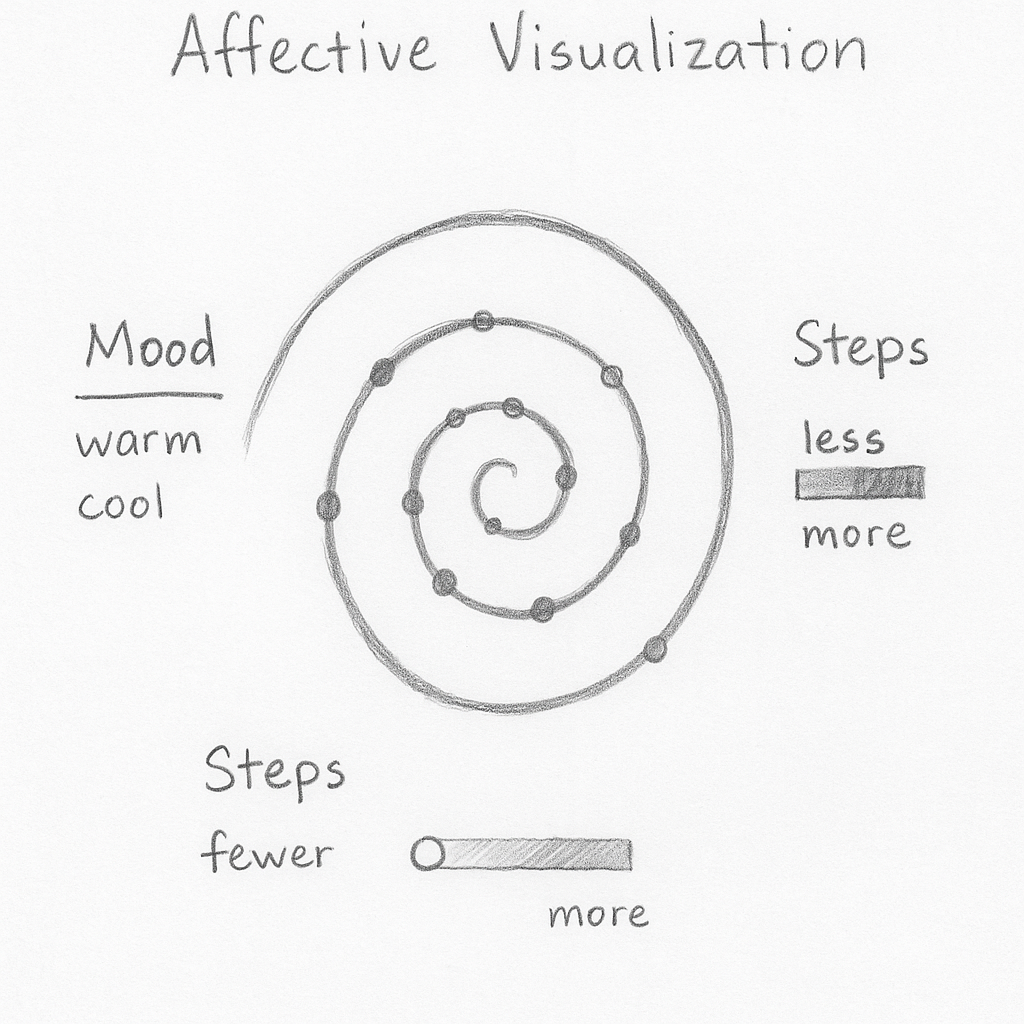
\includegraphics{D:/Git/ENVS-193DS_homework-03/ENVS-193DS_homework-03/Affective Data Spiral Sketch.png}
\#\#\# Problem 2c. Draft of Affective Visualization

Here is a draft of my affective data visualization idea:

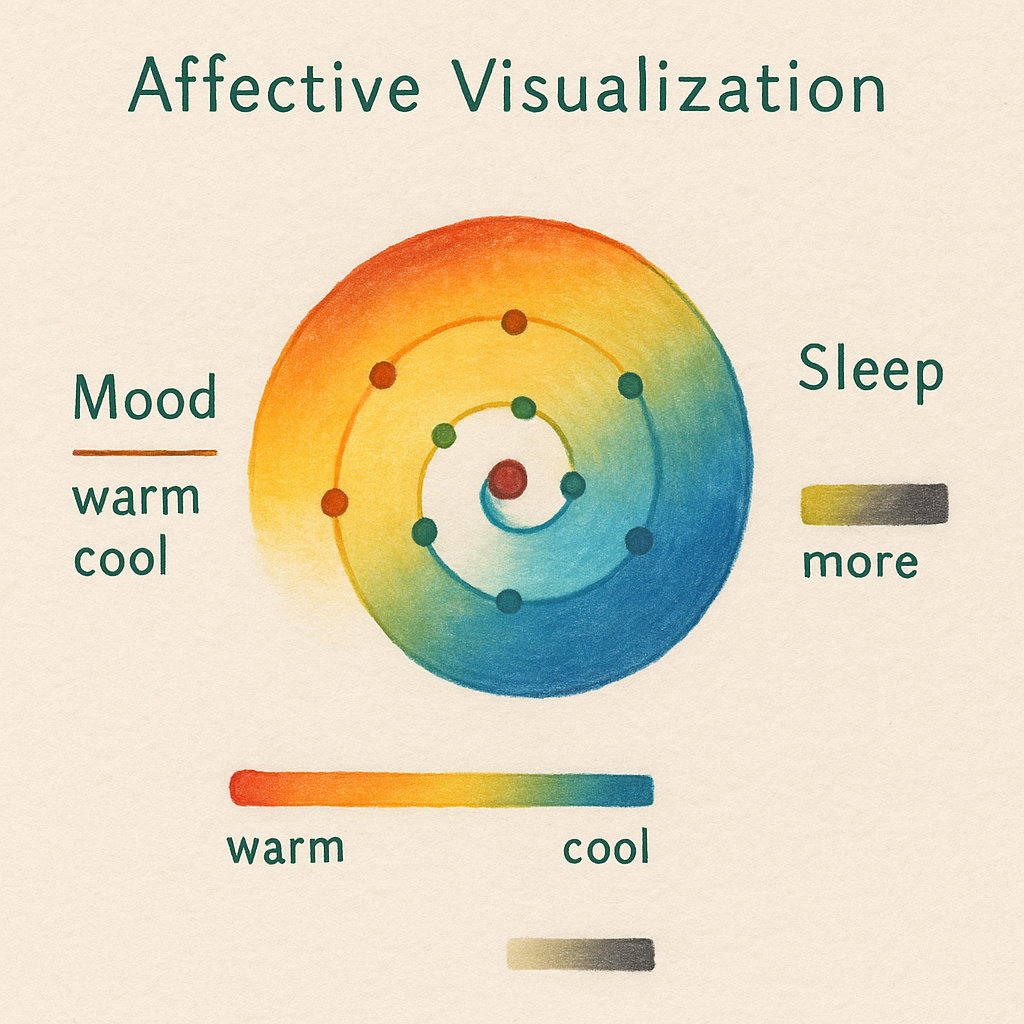
\includegraphics{D:/Git/ENVS-193DS_homework-03/ENVS-193DS_homework-03/New Spiral Image.png}
\#\#\# Problem 2c. Artist Statement

This piece visualizes the relationship between my mood, physical
activity (steps), and sleep patterns over a week. Each layer of the
spiral represents a day, with colors shifting from warm to cool to
reflect mood changes, dot size indicating step count, and background
shading illustrating sleep duration.

I was particularly influenced by Stefanie Posavec and Giorgia Lupi's
Dear Data project, as well as Jill Pelto's environmental watercolor
work, both of which blend personal data with artistic expression to
evoke emotion and insight.

The form of my work is a digitally crafted spiral visualization styled
to resemble a watercolor painting, created using generative design
tools.

To create this piece, I first analyzed trends in my personal data and
then designed a visual metaphor in the form of a spiral, incorporating
color, shape, and layout to communicate affective qualities like energy,
restfulness, and mood.

\subsection{Problem 3. Statistical
critique}\label{problem-3.-statistical-critique}

In the paper by Caulfield et al.~(2020), the authors use a variety of
statistical tests including ANOVA (Analysis of Variance),
Kruskal-Wallis, and Wilcoxon rank-sum tests. These are used to assess
differences in agroecological metrics---such as species richness,
biomass, or clay content---across different land-use types and
management practices. ANOVA was used when assumptions of normality and
equal variance were met, while the non-parametric Kruskal-Wallis and
Wilcoxon tests were applied when these assumptions were violated. These
tests help the authors evaluate whether environmental, land management,
and land-use variables interact to significantly affect ecological
patterns in agroecosystems.ical critique

The x-axis of the figure represents Elevation (meters above sea level),
while the y-axis shows Clay content as a percentage (\%). The figure
uses a scatterplot format with a fitted line that illustrates the trend.
The main message of the figure is to show a positive correlation between
elevation and clay content---clay content increases with higher
elevation.

The figure does a good job communicating this result. The trend line
adds clarity to the relationship, and the data points are not overly
cluttered. However, the figure could be improved with clearer axis
labels (e.g., including units explicitly) and perhaps a statistical
annotation such as an R² value or p-value to help interpret the strength
of the relationship.

Here is a draft of my affective data visualization idea:

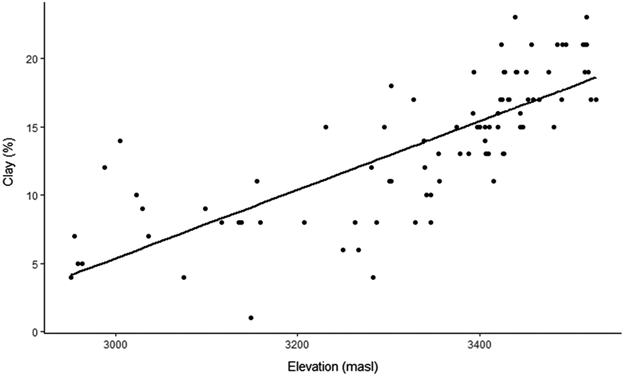
\includegraphics{D:/Git/ENVS-193DS_homework-03/ENVS-193DS_homework-03/homework2crit.png}

\subsection{3b. Visual clarity}\label{b.-visual-clarity}

The authors visually represented their statistics clearly in the figure.
The x- and y-axes are logically positioned and labeled, showing
elevation (meters above sea level) and clay content (\%), respectively.
The scatterplot displays both the raw data points and a fitted
regression line, which effectively communicates the positive
relationship between elevation and clay content. However, the figure
could be improved by including summary statistics such as R² or a
p-value to quantify the strength and significance of the trend.
Additionally, clearer axis titles with units and a legend explaining the
line would enhance interpretation further.

\subsection{3c. Aesthetic clarity}\label{c.-aesthetic-clarity}

The figure handles visual clutter well, with a clean scatterplot layout
and an appropriate number of data points that do not overwhelm the
viewer. The \url{data:ink} ratio is high---most visual elements directly
convey meaningful information, such as the data points and fitted line.
There are no unnecessary gridlines or distracting colors, though adding
subtle visual emphasis (e.g., a contrasting line color or a minimal
legend) could improve clarity further without adding clutter.

\subsection{3d. Recommendations}\label{d.-recommendations}

To improve the clarity and interpretability of the figure, I would
recommend the following enhancements:

Add Summary Statistics: Include the R² value and p-value directly on the
scatterplot. This would allow viewers to immediately assess the strength
and statistical significance of the relationship between elevation and
clay content. These metrics are standard in regression visualizations
and support transparency in data interpretation.

Clarify Axis Labels: While the current axes show the variables, they
should include full units (e.g., ``Elevation (m above sea level)'' and
``Clay Content (\%)'') in a more prominent, bold font to improve
readability and reduce ambiguity for readers unfamiliar with the
variables.

Include a Legend: Add a small legend explaining the meaning of the
regression line (e.g., ``Fitted Linear Trend'') and perhaps distinguish
between observed data points and predicted values if both are shown.
This will help viewers who may not be statistically trained understand
the purpose of each visual element.

Improve Visual Design: Consider enhancing the contrast and color scheme
for accessibility---for example, using colorblind-friendly hues and
slightly increasing the marker size or transparency (alpha) for
overlapping data points to make dense areas easier to read.

Remove Redundant Gridlines: If gridlines are overly dominant or
distracting, reduce their opacity or remove them entirely. This can help
draw focus to the data points and regression line instead of the
background.

\end{document}
